\section{Experimental Setup}\label{sec:setup}
\paragraph{Workload and planners}
Each fixture is a synthetic support ticket requesting one of six business actions over a state with three orders, a customer address, a compensation quota, an escalation status and a ledger. LangGraph~\cite{langchain2025langgraph} alternates model decisions with real tool calls to seven MCP Streamable HTTP services over TLS~1.3/HTTP/2, with request and response bodies padded to 4,096 and 16,384 bytes. Two fixed-weight planners, Qwen3:8B and Llama3.1:8B, run at temperature zero with weights pinned by layer hashes. Each planner executes 300 fixtures per condition: 120 training, 60 validation and 120 paired test fixtures, balanced over the six actions. The label is the requested action, and wrong or failed executions remain in every denominator.

\paragraph{Cover policies}
All four cover arms execute cover on an isolated clone and hide its responses from the real planner; they implement different call-generation strategies (Figure~\ref{fig:dispatch}). \emph{Immediate} cover follows an honest response directly. \emph{History} cover samples a training-only honest gap and service duration, waits in real time and holds the response for the sampled minimum; the \emph{sequential} variant blocks the real chain and the \emph{concurrent} variant overlaps real model inference. \emph{Shadow} runs a complete second planner on an independent ticket whose action is drawn uniformly, and a fair draw decides which chain starts first. Calls to the same service serialize. The shadow also changes call count and composition. Controller positions are fixed before collection among slots after the ticket and up to just after the reference business action; 79/120 test fixtures omit that final slot. Actual issued-call coverage, which also depends on planning and concurrent dispatch, is measured separately in Section~\ref{sec:dispatch}. All no-cover episodes are collected before the cover arms, whose order rotates across fixtures; prompt caches persist across arms. The five conditions give 3,000 main episodes and 600 shadow chains.

\begin{figure}[t]\centering
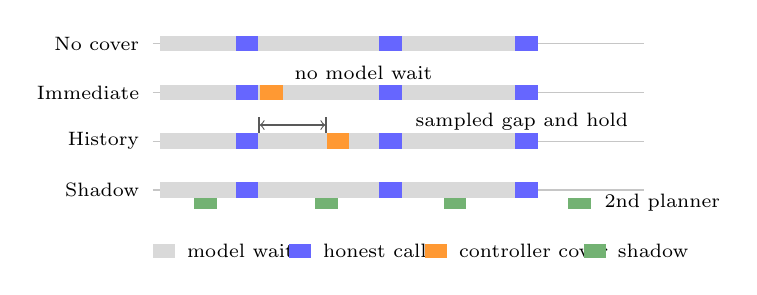
\begin{tikzpicture}[x=.48cm,y=.62cm,font=\scriptsize]
\def\bar#1#2#3#4{\fill[#4] (#1,#3-.16) rectangle (#2,#3+.16);}
\foreach \y/\n in {4/No cover,3/Immediate,2/History,1/Shadow}{
 \node[anchor=east] at (-.1,\y) {\n};
 \draw[gray!45] (0,\y)--(13,\y);
 \bar{0.2}{2.2}{\y}{gray!30}\bar{2.2}{2.8}{\y}{blue!60}
 \bar{2.8}{6.0}{\y}{gray!30}\bar{6.0}{6.6}{\y}{blue!60}
 \bar{6.6}{9.6}{\y}{gray!30}\bar{9.6}{10.2}{\y}{blue!60}}
% immediate cover: right after the honest response
\bar{2.85}{3.45}{3}{orange!80}
\node[anchor=west] at (3.5,3.4) {no model wait};
% history cover: after a sampled gap
\bar{4.6}{5.2}{2}{orange!80}
\draw[|<->|,gray!70!black] (2.8,2.33)--(4.6,2.33);
\node[anchor=west] at (6.7,2.4) {sampled gap and hold};
% shadow chain: its own model waits
\foreach \a in {1.1,4.3,7.7,11.0}{\fill[green!45!black!55] (\a,.62) rectangle (\a+.6,.84);}
\node[anchor=west] at (11.7,.73) {2nd planner};
% legend
\begin{scope}[yshift=-.25cm]
\fill[gray!30] (0,0) rectangle (.6,.3); \node[anchor=west] at (.65,.15) {model wait};
\fill[blue!60] (3.6,0) rectangle (4.2,.3); \node[anchor=west] at (4.25,.15) {honest call};
\fill[orange!80] (7.2,0) rectangle (7.8,.3); \node[anchor=west] at (7.85,.15) {controller cover};
\fill[green!45!black!55] (11.4,0) rectangle (12.0,.3); \node[anchor=west] at (12.05,.15) {shadow};
\end{scope}
\end{tikzpicture}
\caption{Dispatchers in the live study. Honest calls follow a model wait. Immediate cover follows the previous response without one, which label-free gap removal exploits. History-matched cover samples a training gap and response hold. Shadow calls come from a second planner, so their gaps are model waits too.}\label{fig:dispatch}
\end{figure}

\begin{table}[t]\centering\footnotesize
\caption{Study map. Each population answers one question and keeps its own denominators and statistical role.}\label{tab:study-map}
\setlength{\tabcolsep}{3pt}
\begin{tabularx}{\columnwidth}{@{}P{.2\columnwidth}P{.25\columnwidth}Y@{}}\toprule
Study & Population; observer & Question; role \\\midrule
Live timing (\S\ref{sec:dispatch}) & 3,000 episodes + 600 shadow chains; call windows, TLS record times & Does the dispatcher expose cover? Primary families P, R, C \\\addlinespace[2pt]
Feature/role diagnostics & Same episodes; call windows & What changes without time or explicit position? Exploratory refits and saved-prediction strata \\\addlinespace[2pt]
Record-only (\S\ref{sec:noboundary}) & Same episodes; no TEST call boundaries & Original removal pair and later context/joint extension; eight exploratory contrasts \\\addlinespace[2pt]
State control (\S\ref{sec:state}; S1) & 3,600 episodes; call windows, sizes only & Does goal completion miss collateral state? Primary state family \\\bottomrule
\end{tabularx}\end{table}


\paragraph{Studies}
Table~\ref{tab:study-map} lists the populations. The live timing study and its record-only reanalysis answer the privacy questions. A separate earlier state control on the same workload varies termination and feedback across six policies, including a deliberately harmful live-write arm, to test whether goal completion misses collateral state. All runs use one host over loopback with synthetic tools; Section~\ref{sec:limits} states what this does not test.
